% !TeX root = ..\main.tex
% !TeX program = xelatex

% Chapter 1
\chapter{绪论}

本章主要介绍研究背景与意义、中文古诗生成相关的研究现状,阐述本论文的研究思路与主要贡献,并介绍论文的组织架构。

\section{研究背景和意义}

文本生成任务(Text Generation)是自然语言处理(Natural Language Processing, NLP)的一个重要研究方向,需要在给定输入或上下文的条件下,输出符合要求的文本,涵盖机器翻译、文本摘要、对话生成、作品创作等多个应用方向。而在文本生成领域中,中国古代诗歌的生成更是一个困难的任务。

古诗是中华传统文化的瑰宝,作为最早形成的中国古代文学作品体裁之一,其措辞简洁、内涵丰富且韵律整齐。中国古诗的典故意象运用极具文化特色、用词凝练优雅,这些独特的艺术特色都为古诗的机器创作带来巨大的挑战。如何让机器模型深入理解并创作出具有文化内涵和艺术价值的古诗,继而为中华传统文化的再创造赋能,是一个富有挑战的有趣问题。

早期的古诗生成主要依赖于其他子领域的研究思路。例如,基于规则的方法利用现有古诗作为模板,根据既定规则替换字词来生成新的古诗,这样生成的古诗虽在形式上合格,但表达力欠佳\upcite{oliveira2012poetryme};基于摘要的方法将其看作是一个摘要生成任务,只是输入是作者的表达意图,且需要考虑中文古诗独特的韵律形式约束\upcite{yanPoetAutomaticChinese2013};基于统计机器翻译的方法则将其看作一个机器翻译任务,将古诗的上下句子分别看作是翻译的源语言和目标语言,利用统计机器翻译(Statistical Machine Translation, SMT)的方法来生成古诗\upcite{heGeneratingChineseClassical2012}。

随着深度学习技术的发展,近年的中文古诗生成大多将古诗生成视作是“从序列到序列”的预测任务(Sequence-to-Sequence),并由此出发训练循环神经网络(Recurrent Neuro Networks, RNNs),如编码器-解码器(Encoder-Decoder)模型\upcite{yiGeneratingChineseClassical2017},并以此为基础设置额外机制来增强语义表现\upcite{zhangChinesePoetryGeneration2014}或韵律格式约束\upcite{liRigidFormatsControlled2020,huPoetryDiffusionJointSemantic2024}。然而,这些方法对古诗内涵的掌握往往停留在上下文语义或是韵律对仗,无法进一步触达诸如典故、意象和全诗连贯性等更复杂的方面。所幸,大模型(Large Model, LM)展现出强大的语义理解与创作能力,而在中文领域也出现了诸如ERNIE\upcite{zhangERNIEEnhancedLanguage2019}、DeepSeek-R1\upcite{deepseek-aiDeepSeekR1IncentivizingReasoning2025}这样的大语言模型(Large Language Model, LLM)和DeepSeek-VL\upcite{luDeepSeekVLRealWorldVisionLanguage2024}等跨模态大模型,为这一领域注入全新的活力\upcite{yuCharPoetChineseClassical2024}。

除了文本输入外,中国古诗往往蕴含着丰富的场景意象,其对应的视觉信息难以通过用户输入来精确描述。目前也有方案直接使用图像作为输入,如在循环神经网络外增加卷积神经网络(Convolutional Neuro Networks,CNNs)以处理图像信息,捕捉图像关键主体并把握整体氛围,最终生成古诗\upcite{liuImages2PoemGeneratingChinese2018,xuHowImagesInspire2018}。但相应地,这些方案放弃了文本输入能够具体描述要求的优势,输入图像所含信息的繁杂也导致生成古诗主题、内涵乃至风格的波动。现有的方案大都局限于或文本或图像的单一模态输入,要么局限于上下文语义或韵律的形式规律而无法触达更高的艺术层次,要么受制于图像信息的多变而无法实现更精细的输出控制。这种单一模态的输入限制了用户描述需求的可能,也使生成的古诗缺乏层次,这暗示着文图跨模态输入的研究方向,也是本选题希望探讨的内容(如图~\ref{fig:文图生成})。

\begin{figure}[ht]
  \centering
  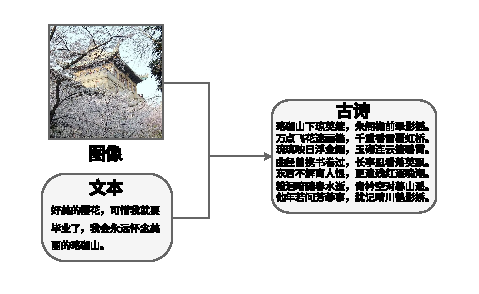
\includegraphics[width=0.8\textwidth]
  {figures/文图生成.pdf}\\
  \caption{文图跨模态的古诗生成}
  \label{fig:文图生成}

\end{figure}

另一个重要的问题是生成结果的“可解释性”(Interpretability),其指系统以人类可理解的术语解释或呈现模型行为的能力\upcite{doshi-velezRigorousScienceInterpretable2017}。深度学习技术在带来更高表现的同时,也因“黑盒”的特性使得可解释性问题愈发突出。在古诗生成任务中,可解释性可体现为三个方面:

\begin{enumerate}[label=(\arabic*), itemindent=2em]   % lefrmargin=2em表示左边距,itemindent=2em表示序号缩进
    \item 过程可解释性,即系统是如何从输入的文本和图像中提取信息,并进一步并生成古诗的,其中包含哪些中间步骤;
    \item 结果可解释性,即系统为何生成这样的古诗结果,其中遵守怎样的韵律形式、又运用了哪些典故意象;
    \item 反馈可解释性,即系统如何分析生成古诗的质量,如何让用户理解古诗“好坏在哪里”。
\end{enumerate}

现有的古诗生成系统大多缺乏对生成过程的可解释性,用户难以理解系统是如何从输入信息中提取出关键信息并生成古诗的。而在结果可解释性方面,现有的系统也往往只提供了生成古诗的文本,而没有进一步解释其韵律、意象等方面的内涵。在反馈可解释性方面,现有的系统也缺乏对古诗质量评价维度的详细说明,用户需要具备较高的文学素养以理解和甄别对古诗质量的评价。因此,提升古诗生成系统的可解释性,将有助于增强用户对系统的信任感和使用体验,使得用户能够更好地理解和利用系统输出的古诗和相应的质量判断。

本文旨在探讨文图跨模态的中文古诗生成,开发了一个基于大模型的古诗创作系统。在给定用户两种模态输入的条件下,其能够通过图像的分析描述来充分提取图像信息,结合用户输入的文本信息,生成符合古诗韵律和意象的古诗。此外,系统还将提供对古诗的分析文本、量化评分以及改进意见,涵盖韵律对仗、典故意象、主题思想、语言用词等多个赏析方面,并支持多轮迭代优化。

\section{研究现状}

下面从与本选题相关的研究现状出发,介绍中文古诗生成、古诗质量评价、大模型技术和提示工程等四个方面的发展状况,为本文工作做铺垫。

\subsection{中文古诗生成}
近年来,中文古诗生成领域引起了广泛的研究兴趣。2016年,为解决古诗生成过程中主题漂移的问题,有研究使用修改的注意力结构的编码器-解码器模型,但限制关键词的数量和顺序,降低了系统的灵活性\upcite{wangChinesePoetryGeneration2016}。这一问题在2018年通过记忆网络(增加记忆组块的RNNs)基于图像生成古诗解决\upcite{xuHowImagesInspire2018}。2020年,有研究将注意力机制引入了Seq2Seq模型,实现了基于关键字的自定义古诗生成\upcite{WangJiYuSeq2SeqMoXingDeZiDingYiGuShiShengCheng2020}。

古诗的生成可能会出现多方面的质量波动,包括主题、语言风格、字数格式、韵律对仗等等,需要在研究中纳入考量。2020年,有研究设计了一个基于Transformer的自回归模型,改进注意力机制并进一步收紧了包括中文古诗、歌词、英文十四行诗等特殊文体生成的格式要求\upcite{liRigidFormatsControlled2020}。2021年,有研究尝试从图像中提取物体关键词、情感和风格,以生成古诗\upcite{wuGenerateClassicalChinese2021}。还有研究将数十万首古诗按照风格、情感、格式与主要关键词分类,并利用掩蔽自注意力机制来建立标签到诗句的关联,以此来生成情感与风格均可控的古诗\upcite{shaoSentimentStyleControllable2021}。到2022年,有研究将GAN中的判别器与生成器结构加入到CVAE中,实现对风格和情感的控制\upcite{LiFengGeHeQingGanKongZhiDeZhongGuoGuShiShengCheng2022}。2023年,有研究构建了一个古诗图像数据集,精确标注了其中的诗歌元素,并利用GRU网络来增强生成古诗的上下文关联\upcite{renGeneratingChinesePoetry2023}。2024年,扩散模型首次被使用来生成古诗,以实现对语义与韵律的同时控制\upcite{huPoetryDiffusionJointSemantic2024}。

后来逐渐出现使用大语言模型生成古诗的方案。2024年,有研究通过强化学习算法PPO对GLM模型进行训练,提升其在古诗生成方面的表现\upcite{CengShengChengShiYuYanMoXingZaiGuShiShengChengZhongDeYouHua2024}。“CharPoet”这一研究则修正了LLM以token计数会导致输出格式错误的问题,改以字符计数,达到了极高的格式精度\upcite{yuCharPoetChineseClassical2024}。还有研究提出了一种图片输入的三段式绝句生成方法,将短语特征纳入考量,并构建了一个图像主题数据集。其将输入的图片映射到一个主题词,再随机选择与该主题词相关的短语,再通过一正一反两种方向的LLM来依次生成古诗的首行、标题和其他主体内容\upcite{liuMultiModalChinesePoetry2018}。

值得注意的是,鲜有研究关注文图跨模态的古诗生成。据调研,目前只有一项研究同时包含文本和图像两种模态的输入,其通过Clarifai来将图像映射到两个具体的主题词,根据这两个主题词在已有短语库中进行检索拓展,再进一步将得到的短语通过一个自注意网络来生成古诗\upcite{liuDeepPoetryChinese2020}。这一系统允许用户来限制古诗的诗句前缀词,因此可广义地认为实现了图文的跨模态输入。

\subsection{古诗质量评价}
如何评价生成古诗的质量是一个难题,考虑到古诗体裁的艺术性,其质量评价往往依赖于人工评估。除此之外,也可使用以往文本生成的自动度量方法,如源自机器翻译领域基于$n$-gram的翻译文本评估方法
BLEU\upcite{papineniBLEUMethodAutomatic2002}和ROUGE\upcite{linROUGEPackageAutomatic2004}($n$-gram表示文本中连续的$n$个词或字符,如“我爱你”中基于字符的$2$-gram集合为[“我爱”、“爱你”])。其中,BLEU指标计算生成文本中有多少$n$-gram出现在参考文本中,即使用精确率(Precision)来评估生成文本有多接近参考文本;相反,ROUGE指标计算参考文本中有多少$n$-gram能够被生成文本包含,即使用召回率(Recall)来评估生成文本能否完整地覆盖参考文本。可见,BLEU和ROUGE指标均依赖于与高质量参考文本的对比。此外,Distinct\upcite{liDiversityPromotingObjectiveFunction2016}基于$n$-gram的多样性来评估生成古诗的多样性,即诗句里有多少不同的$n$-gram。而为了评估上下文语义的一致性,Similarity\upcite{wietingUniversalParaphrasticSentence2016a}使用词向量来计算句子之间的相似度。这些方法都能脱离参考文本独立地评价文本质量。

除了自动度量方法外,也有一些研究通过深度学习模型实现了对古诗的质量优化。2020年,有研究提出一个质量感知的掩蔽语言模型,实现一个可迭代的古诗优化框架,可用于判断古诗是否需要优化,并在润色时定位不恰当部分\upcite{dengIterativePolishingFramework2020}。2023年,有研究提出一种人机协作的古诗创作系统,能够在不同的约束条件下对古诗进行润色\upcite{maYuShengHumaninLoop2023}。2024年,又有研究提出了一个可迭代的古诗优化框架,基于BiLSTM和CRF构建用于检测低质量用词的检测网络、基于BERT模型构建用于修正用词的校正网络\upcite{chenPolishingModelMachineGenerated2024}。这些研究均实现了“评价+优化”的流程功能,且效果良好。美中不足的是未提供对“评价”本身的解释,即“被选中的词为何是低质量的,而优化又依据着什么”的问题。
\subsection{大模型技术}
近年来,大模型技术取得了显著的进步,其中以大语言模型最为典型,例如OpenAI开发的生成预训练转换器(GPT)系列模型、百度开发的知识整合增强表示(ERNIE)系列模型\upcite{zhangERNIEEnhancedLanguage2019}。DeepSeek开发了首个通过强化学习训练的大语言模型 DeepSeek-R1\upcite{deepseek-aiDeepSeekR1IncentivizingReasoning2025},其采用混合专家模型(Mixture-of-Experts, MoE)架构,实现在相同计算成本下大幅提升模型的参数规模与推理能力。

而与LLM擅长自然语言类似,还有许多跨模态大模型适用于不同模态间数据的信息表征处理,如文本和图像。由OpenAI开发的CLIP模型\upcite{radfordLearningTransferableVisual2021}包含一个文本解码器和一个图像解码器,在大量图像及其对应的文本描述的数据集上进行预训练,因而能够把握视觉表征与文本之间的关联。MiniGPT-4\upcite{zhuMiniGPT4EnhancingVisionLanguage2023}是GPT-4模型的缩小版,它将一个与BLIP-2架构相同的视觉编码器与语言模型Vicuna通过一个单一的投影层链接起来,在图像描述生成方面展现出卓越的能力。
DeepSeek开发的DeepSeek-VL\upcite{luDeepSeekVLRealWorldVisionLanguage2024}的训练数据来自广泛的现实场景,其采用了一个混合视觉编码器,可在固定的token预算内有效处理高分辨率图像,同时保持相对较低的计算开销,这一设计选择确保了模型在各种视觉任务中捕捉关键语义和详细信息的能力。有趣的是,DeepSeek-VL在一开始便整合了LLM的能力训练,促进视觉和语言两种模态能力的平衡整合,使其在能够捕捉视觉语义信息的同时,仍然具有强大的语言能力。在此基础上,DeepSeek-VL2\upcite{wuDeepSeekVL2MixtureofExpertsVisionLanguage2024}进一步改进了视觉与文本的能力整合。视觉上融入动态分块的编码策略以处理不同比例尺寸的图像,文本上则引入了MoE架构,可动态选择专家模型完成不同的任务。

\subsection{提示工程}
提示工程逐渐作为一种通过自然语言来调整和控制LLM行为的技术。目前人们已提出多种提示词的设计原则与策略:Few-shot框架\upcite{brownLanguageModelsAre2020}为模型提供少量示例样本,以有效地指示模型完成指定任务。思维链(CoT)框架\upcite{weiChainofThoughtPromptingElicits2022}指导模型将任务分解为若干子任务来逐步完成,使模型能在无其他修改的情况下完成复杂的因果推理任务。自洽性(Self-Consistency)\upcite{wangSelfConsistencyImprovesChain2023a}旨在小样本CoT中对多种推理路径进行采样,并在尝试生成之后选择最一致的答案,其有助于提高CoT提示在涉及算术推理和常识推理的任务中的性能。此外,开发者们也提出了十分多样的提示词框架,例如CRISPE\upcite{crispe}、ICIO、BROKE,均经过了开源社区的检验,令人目不暇接。

\section{研究思路和主要贡献}

本选题旨在利用大模型的通用能力,设计并实现一个文图跨模态的中文古诗创作系统,使其能够:1)分析输入的图像,生成易使用的描述文本,兼顾关键物体与整体氛围;2)生成高质量的古诗,同时给出赏析、典故注释和白话文翻译,提高结果的可解释性;3)对生成古诗进行评分,从多个维度解析古诗的质量,并给出改进建议;4)对生成的古诗进行改进,在不脱离用户输入需求的前提下进行优化。研究内容如图~\ref{fig:研究内容}所示。


\begin{figure}[ht]
  \centering
  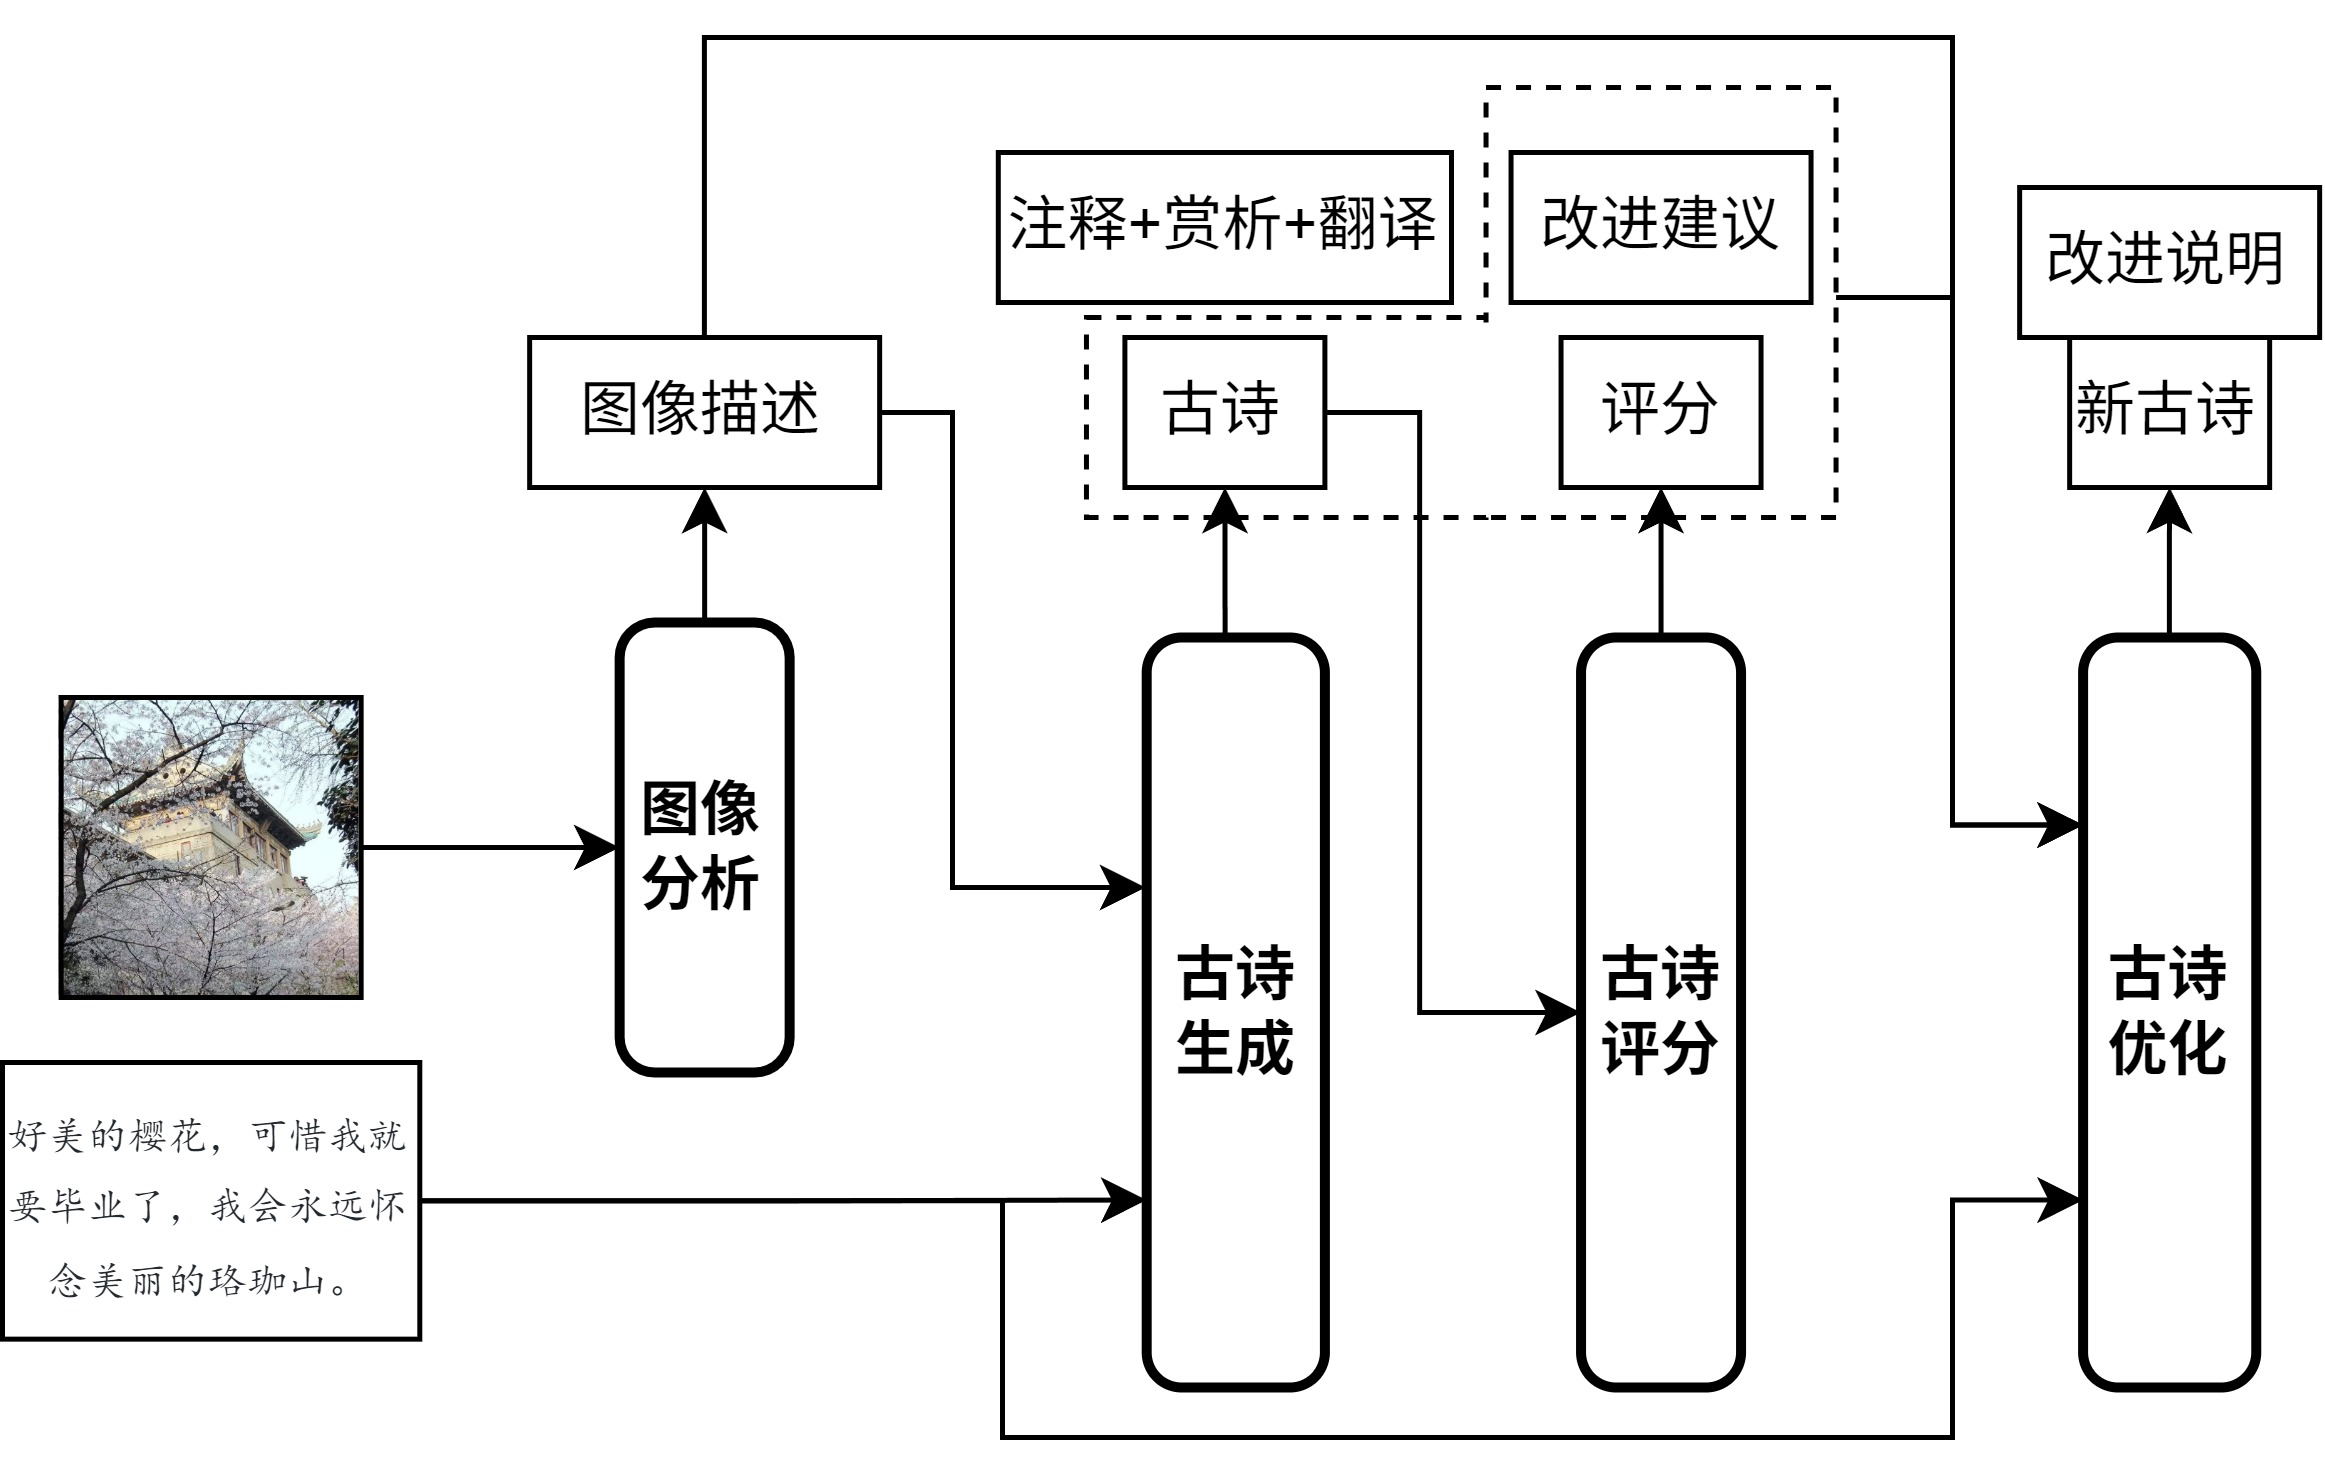
\includegraphics[width=1\textwidth]
  {figures/研究内容.jpg}\\
  \caption{研究内容}
  \label{fig:研究内容} % 添加标签
\end{figure}

为处理输入的图像模态,需要使用跨模态能力优良的视觉与文本编码模型,能够为图像生成描述文本,对图像中的物体特征、空间信息和整体氛围进行充分描述。而由于这段图像描述会用于后续的古诗生成,模型还需要能识别出图片中的文化符号和隐含的情感信息,能够与中国传统文化要素产生勾连,输出的描述文本也应当体现出这些信息。

为输出符合格律要求的古诗,需要设计提示词来指导和约束模型的输出。而为了让输出的古诗不仅符合韵律要求,还能展现出古诗的意境和典故,并且在注释、赏析、白话文翻译等附加文本中进行用户友好的解释,需要使用对典故意象方面理解与运用能力较强的模型。

为有效地评估生成古诗的质量,需要设计合理科学的评分体系,将古诗的质量划分为不同的维度,对不同维度下的不同给分区间进行举例描述。根据体系获得的评分应当能给出具有区分度的分数,以有效反映古诗的质量,还应针对表现欠佳的维度给出针对性的修改意见,以供后续优化使用。

为有效改进生成的古诗,需要参考改进意见来对古诗进行针对性修改。但同时,为了避免优化时忽略其他方面的考虑、导致其他维度的分数降低,需要同时参考原古诗的评分。同理,为了避免优化过程不偏离用户的原始意图,还需要将文本输入与图像描述纳入考量。如此,系统对原古诗的改进将兼顾作品质量和用户需求。

本文使用DeepSeek-VL模型来进行图像分析,相比于英文模型CLIP与MiniGPT4更能捕捉图像中潜在的文化意味与情感,生成的图像描述文本更具诗意美感,且在古诗生成的质量上也更具优势。古诗生成、评分与优化则使用基于强化学习训练的DeepSeek-R1模型,其链式的推理过程包含对多种候选推理路径的动态评估和筛选,能够在反复验证中确保生成古诗的韵律要求,并且也展现了比ERNIE-4.0模型更强的典故意象运用能力。为有效地评估生成古诗的质量,本文设计了一个包含“格律规范”、“意象意境”、“主题思想”、“语言锤炼”、“创新性”等五个维度的评分体系,并附上各分数段的具体例子,有效提升了评分结果的区分度和合理性,也为后续的优化提供了更清晰的方向。而作为补充,本文也将利用BLEU、ROUGE、Distinct、Similarity等指标作为辅助评估。

此外,本文还设计了一系列实验来检验系统的功能,包括不同模型生成古诗的能力对比,古诗评分功能的有效性检验,以及文图跨模态输入对生成古诗的影响。通过这些实验,本文验证了系统功能的有效性,并为后续研究提供了参考。

本文的主要贡献在于:1)结合文图两种模态来强化生成古诗与用户需求的契合度,基于DeepSeek-R1输出既符合格律要求、又富有典故意象的高质量古诗;2)在生成古诗时,输出注释等用户友好的解释性文本,提高了系统输出结果的可解释性;3)设计维度合理、标准明确的古诗评分体系,实现了可解释性强的古诗评分,且相比于自动度量方法更稳定;4)结合用户输入和评价结果,实现了兼顾作品质量与用户意图的古诗优化。此外,本文还测试探索不同大模型在图像描述和古诗生成上的表现,尤其是对诗意美学和意象典故的把握,并讨论了文图跨模态输入对生成古诗的影响。

\section{论文组织结构}

    第一章是概论部分。
    
    第二章介绍古诗生成任务的现有技术,对古诗的基本要求、自动度量方法、DeepSeek大模型等进行概述。

    第三章介绍本系统的设计与实现,包括系统整体架构、各个模块的功能和实现方法。

    第四章介绍开展实验的设计与结果分析,基于已有古诗数据集,结合自动度量方法来评估系统,并展开分析论述。

    第五章是结语,对本文的工作内容进行总结,并探讨局限性与改进空间。
  